\section{Study Design}
\paragraph{Observational Studies}
\textsl{Case-Control Studies}: Split by response $\Rightarrow$ What was done differently in the PAST? (Retrospective)\\
\textsl{Sample Surveys}: What does the population look like NOW? (Cross-Sectional)\\
\textsl{Cohort Studies}: Identify a group now $\Rightarrow$ Observe in the future. (Prospective)\\
\textcolor{OliveGreen}{Pros:}
\begin{itemize}
	\item Ethical and Easier to conduct
	\item Availability of Data
	\item Causality is not always required information
\end{itemize}
\textcolor{Bittersweet}{Cons:}
\begin{itemize}
	\item Not possible to establish cause and effect
	\item Lurking Variables can affect the results
\end{itemize}
Consistent concusion of observational studies $\Rightarrow$ \textcolor{Bittersweet}{Probable} causal
relationship but \textcolor{Bittersweet}{never definitely!}\\
\paragraph{Conducting a Sample Survey}
\begin{enumerate}
	\item \textcolor{Blue}{Sampling Frame}: List of subjects for sampling\\
		$\Rightarrow$ Ideally = Population
	\item \textcolor{Blue}{Sampling Design}: Method of subject selection\\
		$\Rightarrow$ Ideally sampled by chance
		\begin{itemize}
			\item Simple Random Sampling
			\item Cluster Random Sampling\\
				\textcolor{OliveGreen}{\textsl{Use when:}}
				\begin{itemize}
					\item Reliable frame unavailable
					\item Cost of SRS too high
				\end{itemize}
				\textcolor{Bittersweet}{\textsl{BUT}}
				\begin{itemize}
					\item Larger sample size required
					\item Selecting small number of clusters might be more
					homogeneous than population
				\end{itemize}
			\item Stratified Random Sampling\\
				\textcolor{OliveGreen}{\textsl{Use when:}}
				\begin{itemize}
					\item Response differs typically across strata
					\item To include enough subjects in each stratum
				\end{itemize}
				\textcolor{Bittersweet}{\textsl{BUT}}
				\begin{itemize}
					\item Must know the stratum each subject belongs to
					\item Need to define multiple sampling frames
				\end{itemize}
		\end{itemize}
		$\Rightarrow$ Non-Random Sampling sometimes required
		\begin{itemize}
			\item Convenience Sample
				\begin{itemize}
					\item Data can be obtained relatively \textcolor{OliveGreen}{cheaply}
					\item May \textcolor{Bittersweet}{poorly} represent the population
					\item Bias depends on the method of convenience sample
				\end{itemize}
			\item Volunteer Sample
		\end{itemize}
		\begin{Figure}
			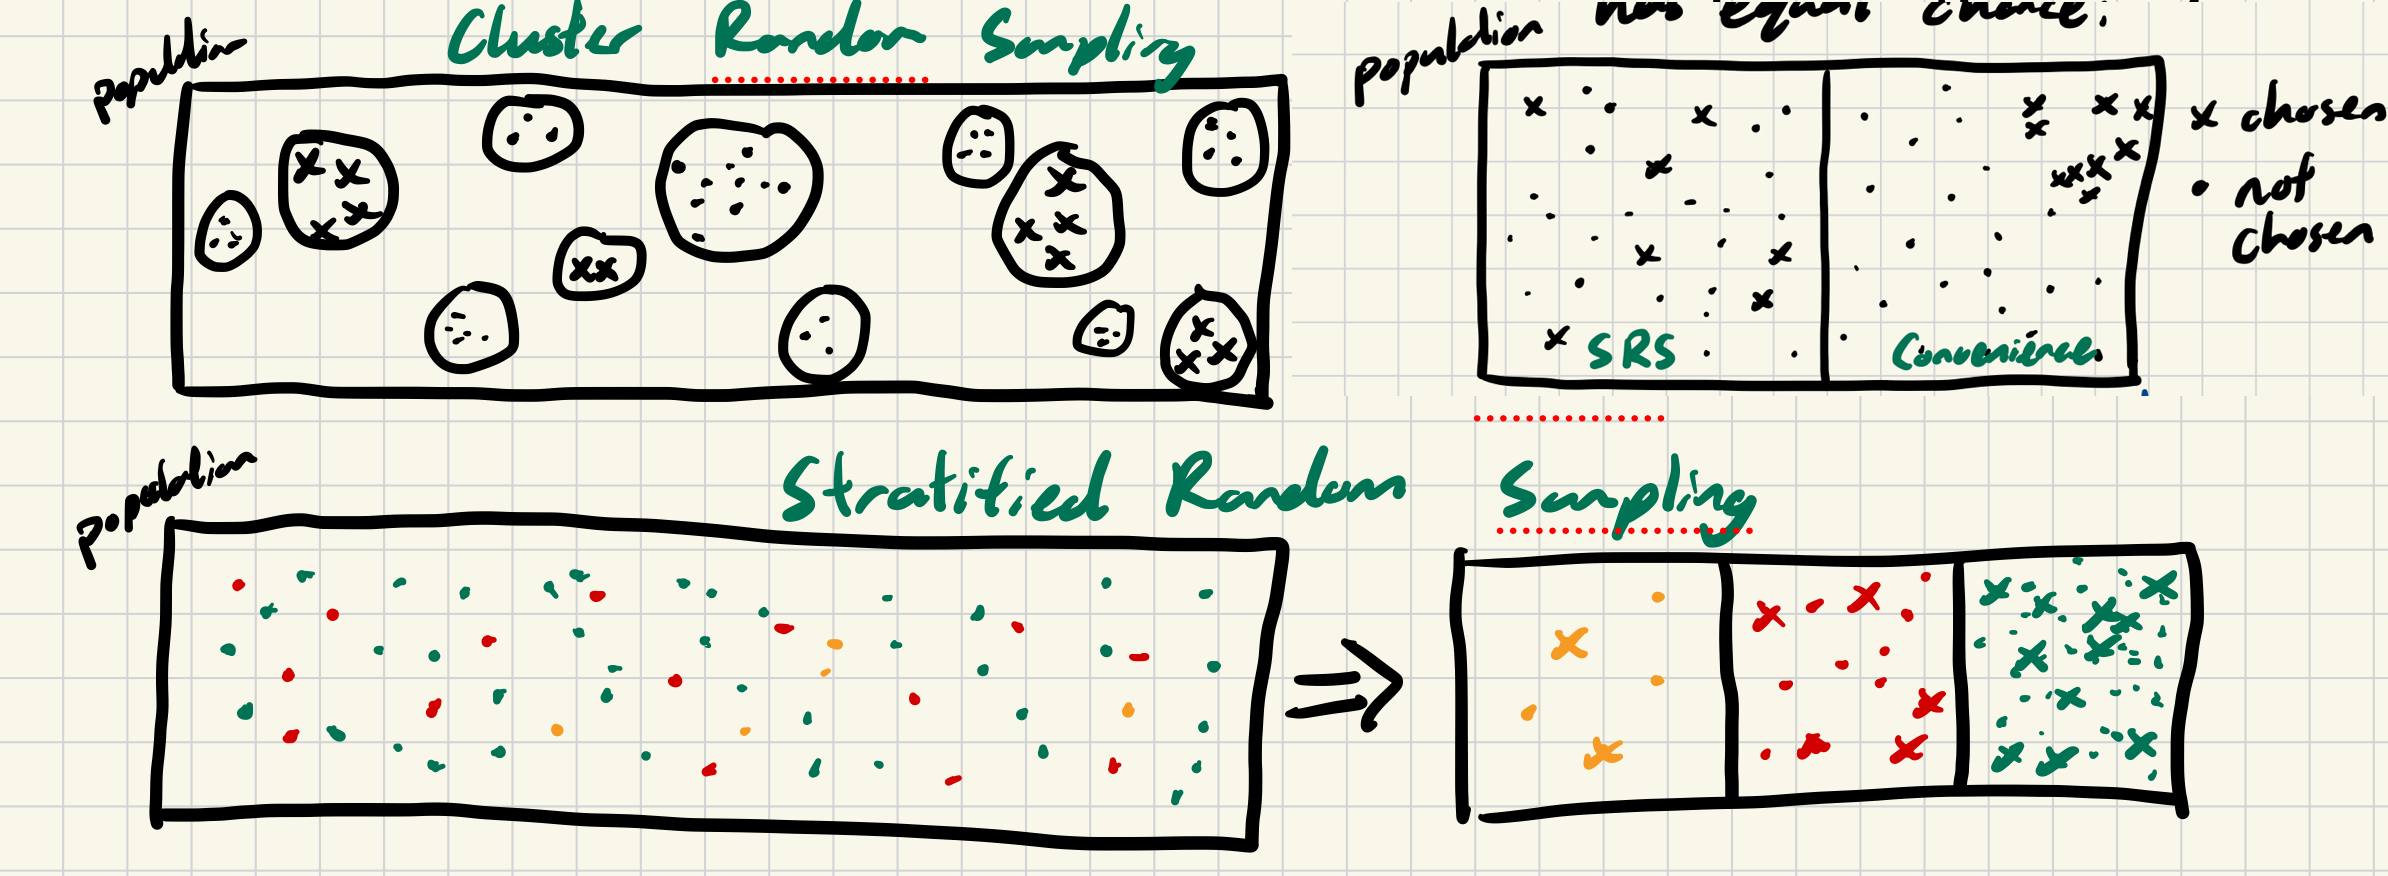
\includegraphics[width=\linewidth]{samplingDesigns.png}
		\end{Figure}
	\item \textcolor{Blue}{Data Collection}
\end{enumerate}
\begin{tabular}{p{0.26\linewidth} p{0.25\linewidth} p{0.26\linewidth}}
	F2F Interview&Phone Interview&Self-Admin Questionnaire\\
	\toprule
	More likely to participate&Less patient, likely to hang up&Lower participation rates\\
	\midrule
	High costs&Low costs&Low costs\\
	\midrule
	May not answer sensitive questions on opinion and lifestyle&&More willing to answer sensitive questions\\
	\bottomrule
\end{tabular}
\textbf{Sampling Bias}: Bias during sampling
\begin{itemize}
	\item Non-Random Sampling
	\item Undercoverage: Non-representative sampling frame\\
		\textcolor{Blue}{eg. Survey through landlines not reaching homeless people}
\end{itemize}
\textbf{Non-Sampling Bias}: Bias during data collection
\begin{itemize}
	\item Nonresponse Bias
		\begin{itemize}
			\item Sampled subjects cannot be reached/refuse to participate
			\item Missing data for certain questions
		\end{itemize}
	\item Response Bias
		\begin{itemize}
			\item Non-honest responses
			\item Confusing/Leading questions
			\item Answering wrongly
		\end{itemize}
\end{itemize}
\paragraph{Experimental Studies}
\begin{itemize}
	\item More sure of a causal relationship as lurking variables' impacts more easily addressed.
	\item Random selection of treatments $\Rightarrow$ Reduced potential for lurking variables.
\end{itemize}
\paragraph{Conducting an Experiment}
\begin{enumerate}
	\item Obtaining experimental units\\
		Typically have to be a convenience sample\\
		$\Rightarrow$\textcolor{Bittersweet}{Representative?}
	\item Assigning to treatments\\
		\textcolor{Blue}{The Control Group}: Placebo/Existing treatments for ethical or comparison reasons\\
		\textcolor{Blue}{Random Assignment}:
		\begin{itemize}
			\item Prevent bias with systematically different non-randomly assigned groups\\
			\item Balance groups on lurking variables to prevent effects on association
		\end{itemize}
	\item Performing Treatment\\
		\textcolor{Blue}{Blinding}: Units unaware of treatment\\
		\textcolor{Blue}{Double-Blinding}: Those in contact with units unaware of treatment
\end{enumerate}
